

\tikzset{every picture/.style={line width=0.75pt}} %set default line width to 0.75pt        

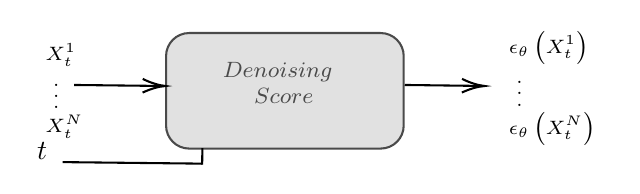
\begin{tikzpicture}[x=0.75pt,y=0.75pt,yscale=-1,xscale=1]
%uncomment if require: \path (0,300); %set diagram left start at 0, and has height of 300

%Rounded Rect [id:dp24071416230204656] 
\draw  [color={rgb, 255:red, 74; green, 74; blue, 74 }  ,draw opacity=1 ][fill={rgb, 255:red, 155; green, 155; blue, 155 }  ,fill opacity=0.3 ] (168.2,80.57) .. controls (168.2,74.42) and (173.18,69.43) .. (179.33,69.43) -- (271.57,69.43) .. controls (277.72,69.43) and (282.7,74.42) .. (282.7,80.57) -- (282.7,113.97) .. controls (282.7,120.12) and (277.72,125.1) .. (271.57,125.1) -- (179.33,125.1) .. controls (173.18,125.1) and (168.2,120.12) .. (168.2,113.97) -- cycle ;
%Straight Lines [id:da22602744857176815] 
\draw    (123.87,94.45) -- (165.87,94.93) ;
\draw [shift={(167.87,94.95)}, rotate = 180.65] [color={rgb, 255:red, 0; green, 0; blue, 0 }  ][line width=0.75]    (10.93,-3.29) .. controls (6.95,-1.4) and (3.31,-0.3) .. (0,0) .. controls (3.31,0.3) and (6.95,1.4) .. (10.93,3.29)   ;
%Straight Lines [id:da9408345556253781] 
\draw    (283.2,94.45) -- (319.7,94.92) ;
\draw [shift={(321.7,94.95)}, rotate = 180.74] [color={rgb, 255:red, 0; green, 0; blue, 0 }  ][line width=0.75]    (10.93,-3.29) .. controls (6.95,-1.4) and (3.31,-0.3) .. (0,0) .. controls (3.31,0.3) and (6.95,1.4) .. (10.93,3.29)   ;
%Straight Lines [id:da18925853941384863] 
\draw    (118.32,131.62) -- (185.7,132.36) ;
%Straight Lines [id:da39360099253546355] 
\draw    (185.7,124.93) -- (185.6,132.81) ;

% Text Node
\draw (102.03,73.02) node [anchor=north west][inner sep=0.75pt]  [font=\scriptsize]  {$ \begin{array}{l}
X_{t}^{1}\\
\ \vdots \\
X_{t}^{N}
\end{array}$};
% Text Node
\draw (325.2,67.35) node [anchor=north west][inner sep=0.75pt]  [font=\scriptsize]  {$ \begin{array}{l}
\epsilon _{\theta }\left( X_{t}^{1}\right)\\
\ \vdots \\
\epsilon _{\theta }\left( X_{t}^{N}\right)
\end{array}$};
% Text Node
\draw (221.94,94.45) node  [font=\footnotesize]  {$ \begin{array}{l}
\textcolor[rgb]{0.29,0.29,0.29}{Denoising}\\
\textcolor[rgb]{0.29,0.29,0.29}{\ \ \ \ Score\ }
\end{array}$};
% Text Node
\draw (104.57,120.8) node [anchor=north west][inner sep=0.75pt]    {$t$};


\end{tikzpicture}
